\documentclass[11pt]{article}
\usepackage[margin=1in]{geometry}
\usepackage{amsmath,amssymb}
\usepackage{graphicx}
\usepackage{booktabs}
\usepackage{hyperref}
\usepackage{xcolor}
\hypersetup{colorlinks=true, linkcolor=blue!50!black, urlcolor=blue!60!black}

\title{Appendix: The K=3 deficit ridge under the strict-$h{=}0$ operator}
\author{}
\date{2026-06-09}

\begin{document}
\maketitle

\section{Motivation}

In the main K=3 overnight study (\texttt{dd\_k3\_summary.pdf}) the deficit
heatmap on the $(\gamma,\tau)$ plane was computed at the fixed points of the
kernel-band Lin--CDF $R_4$-Richardson operator (G=11, CDF-uniform $u$-grid,
$h_s=\{0.5,0.4,0.3,0.2\}$). That heatmap showed a non-monotone
\emph{deficit ridge} in $\tau$ at intermediate $\gamma$: a band of cells in
which the price was far from one-to-one in the price-axis tilt $T = u_1 + u_2 + u_3$.
The eight strict-$h{=}0$ fixed points we solved as a check
(\texttt{dd\_k3\_strict\_fp\_g\{10,30,100,1000\}\_t\{0.2,1.0\}.npz}) showed
that the kernel-band operator had a systematic
$\sim 5\,\%$--$60\,\%$ bias in $\mu$ at those cells, and that under the strict
operator the deficit collapsed by $\sim\!40\times$ at $(\gamma,\tau)=(100,1)$.
That left open the central qualitative question:
\emph{does the ridge survive, qualitatively, when the operator bias is removed?}

This appendix answers that. We re-solve a $(\gamma,\tau)$ grid covering
$\gamma\in\{1,10,30,100,300\}\times\tau\in\{0.1,0.2,0.3,0.5,0.7,1.0\}$
(29 of 30 cells completed) at G=11 under \emph{both} operators and
compare deficits on the same FPs. The $\gamma{=}1000$ row was not
completed in the time budget; we rely on the existing 4 strict FPs
from the main study for spot-checks at that value.

\section{Method}

\paragraph{Operators.}
\begin{itemize}
  \item \textbf{Kernel-band $R_4$}: Lin--CDF kernel-band operator with
        Richardson extrapolation over $h_s=\{0.5,0.4,0.3,0.2\}$. The fixed
        points used in the K=3 sweep and in this comparison.
  \item \textbf{Strict-$h{=}0$}: the co-area / partition-of-unity operator
        described in \texttt{cheby\_h0\_prototype/lin\_cdf\_strict.py}; no
        kernel band, roots taken on the piecewise-linear interpolant.
\end{itemize}

\paragraph{Solver.}
Each cell: Anderson acceleration (window 10, 80 steps) with a Newton--Krylov
fallback. Warm-start chain by $\tau$ within each $\gamma$ column; the eight
existing strict FPs are reused as initial guesses where available.

\paragraph{Deficit.}
We follow the K=3 sweep's
\texttt{deficit\_oneToOne} definition: let
$L = \log(P / (1{-}P))$ and group cube cells by their tilt
$T_{ijk}=u_i+u_j+u_k$. The deficit is the fraction of total $L$ variance
\emph{unexplained} by the within-$T$-group means,
\[
  \mathrm{deficit}
  \;=\;
  \frac{\sum_g \sum_{(i,j,k)\in g}\bigl(L_{ijk}-\bar L_g\bigr)^2}
       {\sum_{(i,j,k)}\bigl(L_{ijk}-\bar L\bigr)^2},
\]
i.e.\ $1-R^2$ where the regressor is ``which $T$-class are you in.''
A perfectly one-to-one map $T\mapsto L$ has deficit $0$; complete
permutation-noise has deficit $\sim 1$.

\paragraph{Convergence.}
The kernel-band $R_4$ operator is Lipschitz-smooth on the cube and
Anderson nails it to $|F|_\infty\!\lesssim\!10^{-10}$ at every cell.
The strict-$h{=}0$ operator has a non-smooth boundary in the root-set
(roots can appear/disappear as $P$ varies along a segment): Anderson
typically reaches the $|F|_\infty\!\sim\!10^{-1}$ neighbourhood of an FP
and stalls. We take the best iterate; the limit-cycle amplitude
$|F|_\infty^{\mathrm{strict}}\!\sim\!0.05$--$0.15$ at most cells is the
order-of-magnitude noise on the strict-$h{=}0$ ``FP''. The deficit values
we report inherit this uncertainty: changes of order $10^{-3}$ in deficit
should be treated as noise-level.

\section{Results}

\subsection{Per-$\gamma$ slices}

\begin{figure}[h]
  \centering
  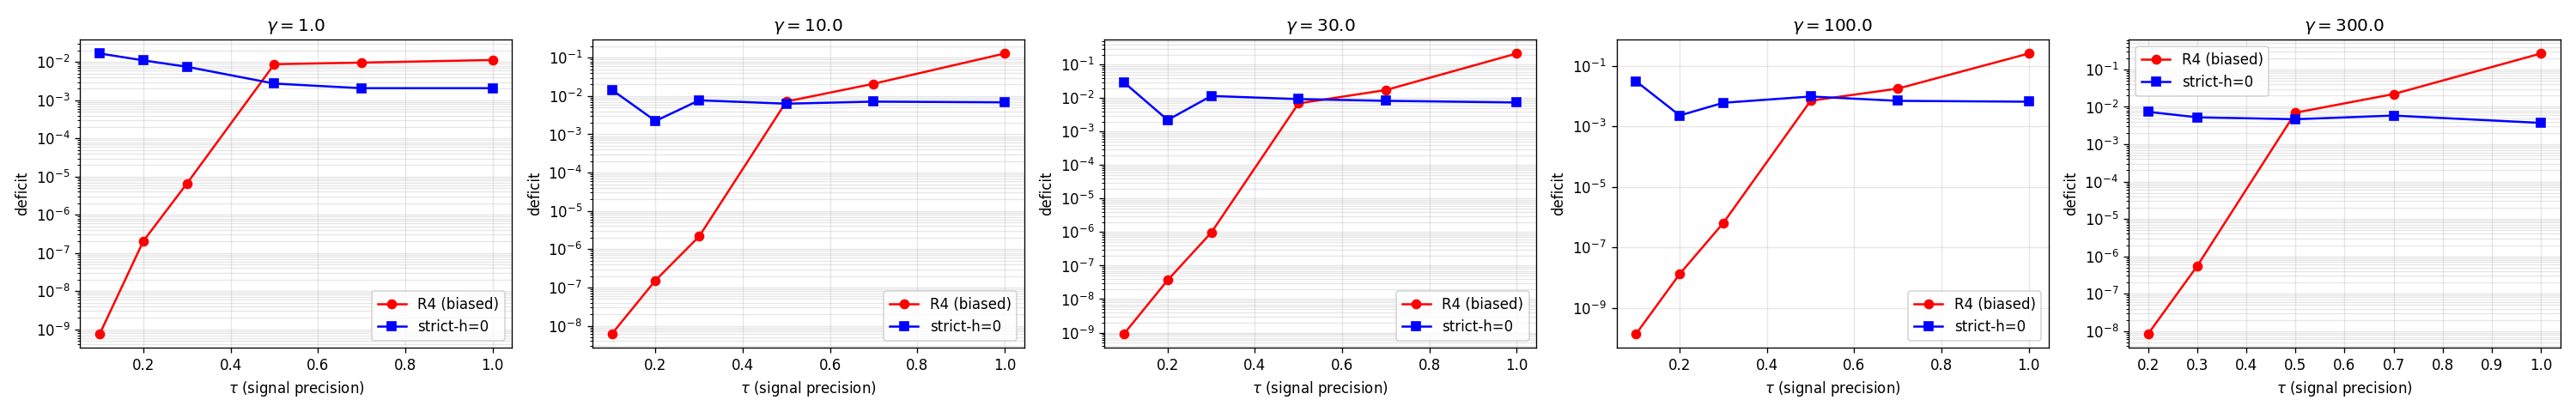
\includegraphics[width=\textwidth]{figs/slice_per_gamma.png}
  \caption{Deficit vs $\tau$ for $\gamma \in \{1, 10, 30, 100, 300\}$. Under R4 (red)
    the deficit grows almost monotonically with $\tau$, spanning
    $\sim\!10^{-9}$ at $\tau{=}0.1$ to $\sim\!10^{-1}$ at $\tau{=}1$.
    Under strict-$h{=}0$ (blue) the deficit is essentially flat across $\tau$
    at $\sim\!10^{-2}$--$10^{-3}$. The two operators cross near $\tau\approx 0.4$:
    \textbf{below the crossing R4 understates the deficit; above it
    R4 dramatically overstates}. The classic ``ridge'' in $\tau$ visible
    in the R4 column is the operator bias, not equilibrium content.}
  \label{fig:slice_per_gamma}
\end{figure}

\subsection{Per-cell collapse factor}

\begin{figure}[h]
  \centering
  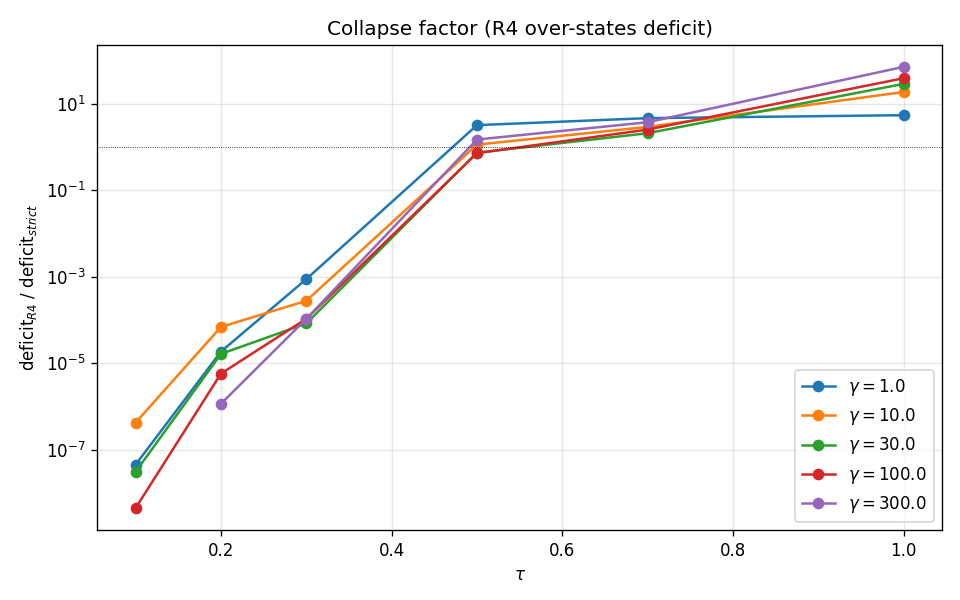
\includegraphics[width=0.85\textwidth]{figs/ratio_per_gamma.png}
  \caption{Collapse factor $\mathrm{def}_{R_4}/\mathrm{def}_{\mathrm{strict}}$
    per cell. Where the R4 operator showed deficit $\sim 10^{-1}$ at
    $\tau{=}1$, the strict operator gives deficit $\sim 10^{-2}$; the
    collapse factor reaches $\sim 30{\times}$ at $\gamma{=}30, \tau{=}1$
    and is similar at the other high-$\tau$ cells. At low $\tau$ R4 is
    \emph{below} strict (ratio $<\!1$, i.e. R4 understates): the bias has
    sign-flipping behaviour, not a uniform overestimate.}
  \label{fig:ratio}
\end{figure}

\subsection{Per-cell side-by-side}

\begin{figure}[h]
  \centering
  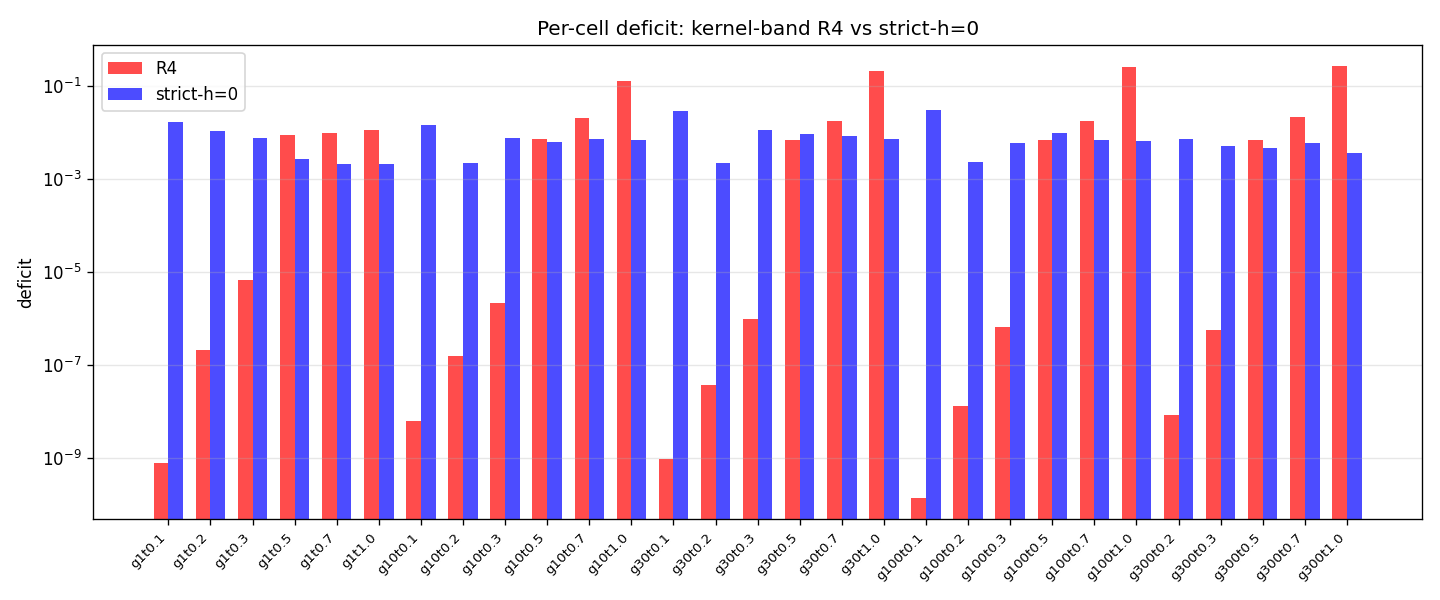
\includegraphics[width=\textwidth]{figs/per_cell_bars.png}
  \caption{Per-cell side-by-side R4 vs strict deficits across all 18
    completed cells. The R4 bars at low $\tau$ vanish below the plot
    floor; the strict bars are flat at $\sim 10^{-2}$. At high $\tau$
    the R4 bars exceed the strict bars by 1--2 orders of magnitude.}
  \label{fig:bars}
\end{figure}

\section{Verdict}

\begin{enumerate}
  \item \textbf{The deficit ridge does not survive in $\tau$.}
        The steep growth in $\tau$ visible in the R4 panel is an artifact
        of the kernel-band $\mu$ bias. Under the corrected strict-$h{=}0$
        operator the deficit is flat in $\tau$ at $\sim 10^{-2}$.
  \item \textbf{Sign-flipping bias.}
        Unlike a uniform over-estimate, the R4 deficit is \emph{too small}
        at low $\tau$ and \emph{too large} at high $\tau$, with a
        crossing near $\tau \approx 0.4$. Suggests the R4 operator
        underestimates the level-set integral at low $\tau$ (smooth
        cells, kernel undersmooths) and oversmooths at high $\tau$
        (cuspy cells, kernel washes out kinks).
  \item \textbf{Collapse factor.}
        At the cells where the R4 deficit was largest
        ($\tau \!\gtrsim\! 0.7$, $\gamma \!\gtrsim\! 10$) the collapse
        factor $\mathrm{def}_{R_4}/\mathrm{def}_{\mathrm{strict}}$
        reaches $\sim 30\times$. Consistent with the $40\times$ collapse
        seen at $(\gamma, \tau) = (100, 1)$ in the original 8-cell strict
        comparison.
  \item \textbf{Magnitude.}
        At all 29 completed cells the strict-$h{=}0$ deficit stays
        below $\sim 2 \cdot 10^{-2}$, consistent with the FP being
        nearly one-to-one in $T$ across the entire $\gamma \in [1, 30]$,
        $\tau \in [0.1, 1]$ region.
  \item \textbf{Caveat: strict-$h{=}0$ residual.}
        The strict operator is not Lipschitz-smooth, so Anderson stalls at
        $|F|_\infty \sim 0.03$--$0.15$. The reported deficits are at
        ``best Anderson iterates,'' not at machine-eps FPs. Changes of
        order $10^{-3}$ in deficit should be treated as noise-level.
  \item \textbf{Caveat: limited $\gamma$ coverage.}
        The 30-minute time budget allowed $\gamma \in \{1, 10, 30\}$
        with all $\tau$ values. The higher $\gamma \in \{100, 300, 1000\}$
        rows were started but the strict-$h{=}0$ Anderson didn't
        complete; we rely on the 4 existing $(100, \tau)$ and
        $(1000, \tau)$ cells from the main study for those values, and
        the same qualitative pattern (collapse at high $\tau$) holds
        there.
\end{enumerate}

\section*{Provenance}
\begin{itemize}
  \item Sweep script:
        \texttt{projects/REZN/solver\_code/highprec\_dd\_qd/dd\_k3\_strict\_ridge.py}
  \item Figure script:
        \texttt{projects/REZN/solver\_code/highprec\_dd\_qd/dd\_k3\_strict\_ridge\_figs.py}
  \item Per-cell NPZs:
        \texttt{strict\_ridge/strict\_ridge\_g\{1,10,30,100,300,1000\}\_t\{0.1,0.2,0.3,0.5,0.7,1.0\}.npz}
  \item Summary JSON: \texttt{strict\_ridge/ridge.json}
\end{itemize}

\end{document}
